\documentclass[10pt,a4paper,landscape]{article}
\usepackage{multicol}
\usepackage{calc}
\usepackage{ifthen}
\usepackage[landscape]{geometry}
\usepackage{hyperref}

\usepackage[utf8]{inputenc}

% Fuentes (Fira Sans)
\usepackage[T1]{fontenc}
\usepackage[sfdefault,scaled=.85]{FiraSans}
\usepackage{newtxsf}
\usepackage[scaled=.85]{FiraMono}

% TikZ for UML

\usepackage{tikz-uml}

% Listings for code

\usepackage{listings}
\lstset{basicstyle=\ttfamily\footnotesize,breaklines=true}

% Multiple cols/rows

\usepackage{multirow}

% Checkmarks

\usepackage{amssymb}

% To make this come out properly in landscape mode, do one of the following
% 1.
%  pdflatex latexsheet.tex
%
% 2.
%  latex latexsheet.tex
%  dvips -P pdf  -t landscape latexsheet.dvi
%  ps2pdf latexsheet.ps


% If you're reading this, be prepared for confusion.  Making this was
% a learning experience for me, and it shows.  Much of the placement
% was hacked in; if you make it better, let me know...


% 2008-04
% Changed page margin code to use the geometry package. Also added code for
% conditional page margins, depending on paper size. Thanks to Uwe Ziegenhagen
% for the suggestions.

% 2006-08
% Made changes based on suggestions from Gene Cooperman. <gene at ccs.neu.edu>


% To Do:
% \listoffigures \listoftables
% \setcounter{secnumdepth}{0}


% This sets page margins to .5 inch if using letter paper, and to 1cm
% if using A4 paper. (This probably isn't strictly necessary.)
% If using another size paper, use default 1cm margins.
\ifthenelse{\lengthtest { \paperwidth = 11in}}
	{ \geometry{top=.5in,left=.5in,right=.5in,bottom=.5in} }
	{\ifthenelse{ \lengthtest{ \paperwidth = 297mm}}
		{\geometry{top=1cm,left=1cm,right=1cm,bottom=1cm} }
		{\geometry{top=1cm,left=1cm,right=1cm,bottom=1cm} }
	}

% Turn off header and footer
\pagestyle{empty}
 

% Redefine section commands to use less space
\makeatletter
\renewcommand{\section}{\@startsection{section}{1}{0mm}%
                                {-1ex plus -.5ex minus -.2ex}%
                                {0.5ex plus .2ex}%x
                                {\normalfont\large\bfseries}}
\renewcommand{\subsection}{\@startsection{subsection}{2}{0mm}%
                                {-1explus -.5ex minus -.2ex}%
                                {0.5ex plus .2ex}%
                                {\normalfont\normalsize\bfseries}}
\renewcommand{\subsubsection}{\@startsection{subsubsection}{3}{0mm}%
                                {-1ex plus -.5ex minus -.2ex}%
                                {1ex plus .2ex}%
                                {\normalfont\small\bfseries}}
\makeatother

% Define BibTeX command
\def\BibTeX{{\rm B\kern-.05em{\sc i\kern-.025em b}\kern-.08em
    T\kern-.1667em\lower.7ex\hbox{E}\kern-.125emX}}

% Don't print section numbers
\setcounter{secnumdepth}{0}


\setlength{\parindent}{0pt}
\setlength{\parskip}{0pt plus 0.5ex}


% -----------------------------------------------------------------------

\begin{document}

\raggedright
\footnotesize
\begin{multicols}{3}


% multicol parameters
% These lengths are set only within the two main columns
%\setlength{\columnseprule}{0.25pt}
\setlength{\premulticols}{1pt}
\setlength{\postmulticols}{1pt}
\setlength{\multicolsep}{1pt}
\setlength{\columnsep}{2pt}


\tikzumlset{font=\footnotesize}

\begin{center}
     \Large{\textbf{PDOO temas 1 y 2}} \\
\end{center}

\section{Conceptos básicos}

\subsection{Envío de mensajes entre objetos}

Diferentes formas de ligar un mensaje al método que lo resuelve

\begin{tabular}{@{}ll@{}}
Estática    & Ocurre antes de la ejecución, más eficiente \\
Dinámica  & Ocurre durante la ejecución, más flexible, la usan Java y Ruby \\
\end{tabular}

\subsection{Especificadores de acceso}

\subsubsection{Java}

\begin{tabular}{cccc}
\multirow{2}{*}{Visible en} & \multicolumn{2}{c}{Mismo paquete} & Otro paquete
  \\
                            & Clase & Otra & Otra \\
  private & \checkmark & & \\
  package & \checkmark & \checkmark & \\
  protected & \checkmark & \checkmark & \\
  public & \checkmark & \checkmark & \checkmark \\
\end{tabular}

Se utiliza \textit{protected} por defecto. Hay introspección, ya que se
puede consultar una clase u objeto en ejecución.

\subsubsection{Ruby}

\begin{tabular}{cccc}
Visible en & Desde el propio objeto & Clase & Otra\\
  private & \checkmark & & \\
  protected & \checkmark & \checkmark & \\
  public & \checkmark & \checkmark & \checkmark \\
\end{tabular}

Se utiliza \textit{private} por defecto. Se pueden consultar y modificar las
clases, métodos y variables en ejecución. 

\section{Diagramas UML}

\subsection{Diagramas de clases}

\begin{tikzpicture}[]
  \umlclass{Nombre$^{multiplicidad}$}{
    [visibilidad] nombreAtributo [:tipo[multiplicidad]][=valorInicial] \\
    $\vdots$ \\
  }{
    [visibilidad] nombreMétodo ([lista parámetros])[:tipo retorno] \\
    $\vdots$ \\
  }
\end{tikzpicture}

La multiplicidad de la clase indica el número de instancias que puede tener. La
de un atributo, el número de elementos que tiene. La descripción de la responsabilidad de la clase puede indicarse debajo. La
visibilidad se marca mediante:

\begin{tabular}{@{}ll@{}}
\verb!+!    & Pública \\
\verb!-!  & Privada \\
\verb!~! & Paquete \\
\verb!#!  & Protegida \\
\end{tabular}

Para indicar un atributo o método de clase, lo subrayamos.

\subsubsection{Relaciones entre clases}


\begin{tikzpicture}[baseline=0]
  \umlemptyclass{C1}
  \umlemptyclass[x=2, y=0]{C2}
  \umldep{C1}{C2}
\end{tikzpicture}
\hskip 4pt \parbox{4cm}{
   Relación de dependencia
}

\begin{tikzpicture}[baseline=0]
  \umlemptyclass{C1}
  \umlemptyclass[x=2, y=0]{C2}
  \umlassoc{C1}{C2}
\end{tikzpicture}
\hskip 4pt \parbox{4cm}{
   Relación de asociación
}

En una relación de asociación se puede indicar el número de objetos que se
asocian de cada clase escribiendo encima de la línea con la sintaxis
\textit{vMin...vMax}.

Existen otras asociaciones:

\begin{tikzpicture}[baseline=0]
  \umlemptyclass{C1}
  \umlemptyclass[x=2, y=0]{C2}
  \umlaggreg{C1}{C2}
\end{tikzpicture}
\hskip 4pt \parbox{4cm}{
   Agregación. Una clase representa el `todo` (C1) y otra las `partes` (C2).
 }

 \begin{tikzpicture}[baseline=0]
  \umlemptyclass{C1}
  \umlemptyclass[x=2, y=0]{C2}
  \umlcompo{C1}{C2}
\end{tikzpicture}
\hskip 4pt \parbox{4cm}{
   Composición. Agregación en la que las `todo` (C1)  no tienen sentido sin el
   `partes` (C2).
 }

 Podemos crear una clase asociación cuando una asociación presenta atributos
 propios y tiene que ser modelada como una clase.

 Los \textit{cualificadores de la asociación} son los atributos de algunas de las clases
 que pasa a ser un atributo asociado a la clase del otro extremo. Al emplear
 colecciones para modelar las asociaciones cualificadas, se emplea el
 cualificador como identificador.

 Las restricciones son extensiones de la semántica del lenguaje, añadiendo
 nuevas reglas o modificando las ya existentes. Se representan entre llaves.

 \subsection{Diagramas de paquetes}


\begin{tikzpicture}[baseline=0]
    \begin{umlpackage}{P1}

    \end{umlpackage}
    \begin{umlpackage}[x=2,y=0]{P2}
    \end{umlpackage}
    \umldep{P1}{P2}
\end{tikzpicture}
\hskip 4pt \parbox{4cm}{
   El paquete P1 usa algún elemento del paquete P2
 }

 \begin{tikzpicture}[baseline=0]
    \begin{umlpackage}{P1}

    \end{umlpackage}
    \begin{umlpackage}[x=3,y=0]{P2}
      \umlsimpleclass{A}
    \end{umlpackage}
    \umldep{P1}{A}
    \node[] at (1.3,0.25) {<<import>>};
\end{tikzpicture}
\hskip 4pt \parbox{3cm}{
   El paquete P1 importa la clase A del paquete P2
 }

 La visibilidad de los elementos de un paquete se marca con + (visible dentro y
 fuera) o - (visible sólo en el paquete).

 \subsection{Diagramas de secuencia}

  Muestran de forma visual el orden en el que ocurren los envíos de mensaje
 dentro de una interacción entre objetos. La sintaxis es la siguiente:

 \begin{tabular}{@{}ll@{}}
Participantes & \texttt{nombre : nombreClase} \\
Mensaje  & \texttt{variable = mensaje(arg) : tipo devuelto} \\
\end{tabular}

 \begin{tikzpicture}
   \begin{umlseqdiag}
     \umlobject[class=C1]{o1}
     \umlcreatecall[class=C2]{o1}{o2}
     \begin{umlcall}[op={2:m1()}, return=2.1: valor devuelto]{o1}{o2}
     \end{umlcall}
     \begin{umlcall}[op={3:m3()}]{o1}{o2}
     \end{umlcall}
     \begin{umlfragment}[type=alt, inner xsep=2, label=c]
     \begin{umlcallself}[op=o1()]{o1}
     \end{umlcallself}
     \end{umlfragment}
   \end{umlseqdiag}
 \end{tikzpicture}

 \begin{tabular}{@{}ll@{}}
   create & crea una instancia \\
   m1() & es un mensaje síncrono y devuelve un valor \\
   m3() & es un mensaje asíncrono \\
   o1() & es un mensaje al propio objeto \\
\end{tabular}

 El recuadro con alt es un \textit{fragmento de interacción}, una secuencia de mensajes
 que ocurre bajo determinadas condiciones. Se pueden combinar. Los argumentos de
 los operadores descritos a continuación se indican dentro, entre llaves.

\begin{tabular}{@{}ll@{}}
  alt & Se ejecuta si se cumple la condición \\
  break & Se ejecuta si se cumple la condición y no se continúa \\
  loop & Se realiza arg veces el fragmento \\
  opt & Como alt pero con un solo fragmento \\
\end{tabular}
 
\subsection{Diagramas de comunicación}

Tipos de enlace (objetoX envía mensaje a objetoY)

\begin{tabular}{@{}l@{}l@{}l@{}}
Global \ & \texttt{G}    & \ \  El ámbito de objetoY es superior al de objetoX \\
Asociación \  &  \texttt{A}  & \ \ Existe una relación fuerte y duradera \\
Parámetro \ & \texttt{P} & \ \ objetoY es pasado como parámetro de objetoX \\
  Local \ & \texttt{L}  & \ \ objetoY es referenciado en un método de objetoX \\
  Self \ & \texttt{S} & \ \ objetoX siempre se conoce a sí mismo \\
\end{tabular}

\section{Clases en Java y Ruby}

\subsubsection{Java}
\lstinputlisting[language=Java]{t12cjava.java}

\subsubsection{Ruby}
\lstinputlisting[language=Ruby]{t12cruby.rb}

\end{multicols}
\end{document}
